\chapter{Five Tips for Writing Your First Novel}

This lecture contains no blackboard mathematics, yet it proceeds with a real formal spine. Sanderson begins from a numerical writing target, turns that target into a practical constraint on daily work, and then unfolds five construction rules that move from borrowed outer structure, to character voice, to character pressure, to the large architecture of progress, and finally back to the writer's own working discipline. We should preserve that order, because the lecture does not present five disconnected tricks; it builds a usable method step by step.

\begin{remark}
The displayed formulas in this chapter are transcript-backed summaries or cautious editorial reconstructions. They are not transcriptions of visible board equations.
\end{remark}

\section{Challenge, Permission, and the Five-Hack Setup}

Sanderson opens by setting the practical frame. National Novel Writing Month is a challenge to write a novel in a month, with the novel here being loosely measured by a target of fifty thousand words. The purpose of the exercise is not perfection. It is almost the opposite: to get the writer out of a rut, to force the internal editor into silence, and to produce pages.

That opening matters because it explains why the lecture will sound procedural from the start. We are not being asked to wait for ideal conditions. We are being asked to work under a constraint.

\begin{equation}
\text{NaNoWriMo target}=50{,}000\ \text{words in one month}.
\end{equation}

Sanderson then inserts an important qualification. The challenge is valuable, he says, but it is not sacred. It may fail to fit a given writer's psychology; the writing produced under that pressure may simply be worse than the writing produced without it. This concession is not a retreat. It is what makes the rest of the lecture trustworthy. The challenge is a tool, not a moral duty.

\paragraph{A worked estimate.} Once the target is fixed, the daily pace follows immediately:
\begin{enumerate}
\item Start from \(50{,}000\) words.
\item Approximate the month by \(30\) writing days.
\item Divide.
\item Round the result to a usable working number.
\end{enumerate}

\begin{equation}
\frac{50{,}000}{30}\approx 1{,}667 \approx 1{,}700\ \text{words/day}.
\end{equation}

That estimate will return later, when the lecture shifts from story mechanics to the ordinary discipline of getting words down.

\subsection{Question \& Answer}

\paragraph{Question.} When is this challenge useful, and when should we abandon it?

\paragraph{Answer.} It is useful when we need a strong external constraint to break hesitation, disable over-editing, and make ourselves produce pages. We abandon it when the constraint stops serving the work, when our writing psychology simply does not mesh with it, or when the challenge produces weaker pages than a slower method would.

From here the lecture pivots cleanly: for those who do want to try, Sanderson will offer five hacks, five ways to begin a novel even when preparation is thin.

\section{Borrowing Structure as Training Wheels}

The first hack begins from a familiar impulse. We see a movie, read a story, hear of an event, and think: could we write something like that? Sanderson's move is to convert that admiration into analysis. We do not copy the finished story. We ask what about that kind of story works, what its hallmark scenes are, and what sequence of pressures and resolutions keeps it alive.

\begin{definition}
A borrowed structure is the extracted functional pattern of a story or subgenre, retained while the surface particulars are replaced.
\end{definition}

His main example is the heist. What is attractive about it is not merely crime, but coordination: a crew of people with distinct specialities who come together to achieve a difficult goal. Once we see that, the structure begins to reveal itself.

\begin{equation}
\text{admired story} \to \text{hallmark scenes} \to \text{fundamental structure} \to \text{new novel}.
\end{equation}

In the lecture the heist pattern is sketched almost algorithmically:

\begin{equation}
\text{problem} \to \text{recruitment} \to \text{preparation} \to \text{coordinated resolution}.
\end{equation}

\begin{figure}
\centering
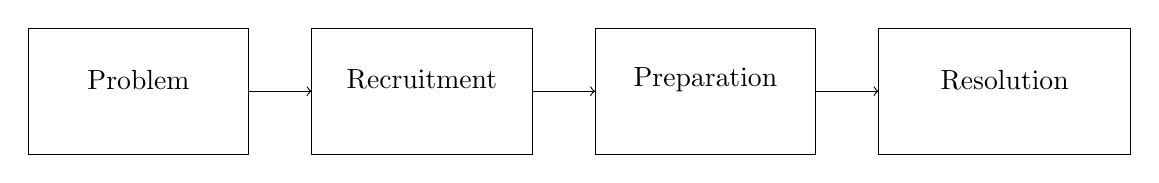
\begin{tikzpicture}
\draw (-5.6,0.8) rectangle (-2.8,-0.8);
\node at (-4.2,0.15) {Problem};

\draw (-2.0,0.8) rectangle (0.8,-0.8);
\node at (-0.6,0.15) {Recruitment};

\draw (1.6,0.8) rectangle (4.4,-0.8);
\node at (3.0,0.15) {Preparation};

\draw (5.2,0.8) rectangle (8.4,-0.8);
\node at (6.8,0.15) {Resolution};

\draw[->] (-2.8,0) -- (-2.0,0);
\draw[->] (0.8,0) -- (1.6,0);
\draw[->] (4.4,0) -- (5.2,0);
\end{tikzpicture}
\end{figure}

This figure is only a transcript-based schematic, but it captures exactly the kind of structural reduction Sanderson is recommending. Once we have boiled a story down to this level, we may rebuild it with new characters, a new problem, and a new character arc. The same method can even be strengthened by transposition. A structure admired in one genre may be moved into another, as when a Regency romance pattern is reimagined as a Western.

\subsection{Question \& Answer}

\paragraph{Question.} How do we borrow a structure without becoming enslaved to it?

\paragraph{Answer.} We borrow only the functional skeleton, not the identity of the original story. We keep the sequence that works, then replace the characters, the world, the problem, and the arc. The borrowed structure acts as training wheels: support, not bondage.

Sanderson is careful here. Professionals do this too. Borrowing structure is not only a beginner's crutch. But it must remain adaptable; the writer must be free to bend it toward the actual story being written.

\section{Beginning with a Monologue}

Once an outer structure is in place, the lecture narrows from architecture to access. How do we get quickly inside a character? Sanderson's second answer is the monologue. Even if the finished book will not be told in first person, we can still ask a character to speak directly and explain a decisive period of life.

\begin{equation}
\text{monologue} \to \text{voice} + \text{history} + \text{usable fragments}.
\end{equation}

The point is discovery. Sanderson cites the practice of asking what a character would say if forced to explain life in five pages. Those five pages may never appear in the final novel. But they teach the writer how that character sounds, what the character notices, what the character hides, and what the character thinks is central.

The lecture then widens this exercise. Material extracted from such monologues may become small chapter-opening blurbs, that is, epigraphs. It may become journal fragments. It may even push the book toward epistolary form.

\begin{definition}
An epistolary novel is a novel written through in-world documents such as journals, letters, or similar records.
\end{definition}

\subsection{Question \& Answer}

\paragraph{Question.} Can a first-person monologue be useful even when the finished novel is not first person?

\paragraph{Answer.} Yes. Here the monologue is not a binding viewpoint choice. It is a discovery instrument. We use it to hear the character clearly, and only afterward do we decide what, if any, of that material belongs in the finished book.

This is a characteristic Sanderson move. A provisional exercise is allowed to remain provisional, but it may also yield finished material if the form proves fertile enough.

\section{Wants, Needs, Obstacles, and Choosing the Right Viewpoint}

The third hack shifts from voice to pressure. Sanderson asks four linked questions: what does the character want, what does the character need, how are those different, and why can the character have neither? At this point the lecture becomes almost dynamical. Plot is no longer treated as something imposed from outside. It is generated from the misfit between outward pursuit and inward necessity.

Let us name the basic objects:
\begin{align}
W&=\text{what the character wants},\\
N&=\text{what the character needs},\\
O&=\text{the obstacles blocking both}.
\end{align}

The lecture's central distinction here is the nonidentity of want and need:

\begin{equation}
W \neq N.
\end{equation}

Once that difference is fixed, the narrative pressure follows from the obstacles that prevent easy access to either:

\begin{equation}
\text{plot pressure}=\text{obstacles to }W\text{ and }N.
\end{equation}

\paragraph{A worked update rule.} Sanderson's procedure for generating plot from character may be written as:
\begin{enumerate}
\item Ask what the character wants.
\item Ask what the character needs.
\item Ask how those differ.
\item Ask why the character cannot simply obtain either one.
\item Turn those answers into obstacles.
\item Let those obstacles determine the early plot.
\end{enumerate}

This is why the lecture insists that the story remain character-centered. If the plot turns on the wants and needs of the viewpoint character, then the character remains inside the machinery of the novel rather than standing outside and commenting.

Sanderson then identifies a common beginner's error. The nominal main character may turn out to be only an observer, while the real drama belongs to somebody else. That is a viewpoint failure. The correct protagonist is not merely the person on the page most often. It is the one for whom the stakes, conflict, and change are largest.

\subsection{Question \& Answer}

\paragraph{Question.} Which character should actually carry the story?

\paragraph{Answer.} Not the passive observer, however convenient that observer may seem. The story should belong to the character who is changing the most, enduring the most conflict, or striving most actively for what is wanted. The viewpoint must be personal to that character, or else the real story will appear to be happening elsewhere.

This prepares the next major pivot. Sanderson now imagines the writer answering all these character questions and still protesting: I understand the character, but I still do not have a structure.

\section{Promise, Progress, Payoff, and the Signposting of Motion}

The fourth hack answers that objection by offering the lecture's clearest formal compression. If Sanderson boils story down to its essential pattern, we obtain three terms:

\begin{equation}
\text{story}=\text{promise} \to \text{progress} \to \text{payoff}.
\end{equation}

The promise names what kind of satisfaction or motion the story offers. The payoff fulfills that promise. But the great middle term, Sanderson insists, is progress. That is the bulk of the story. Readers continue not because the book simply contains events, but because they can feel movement toward something.

\begin{figure}
\centering
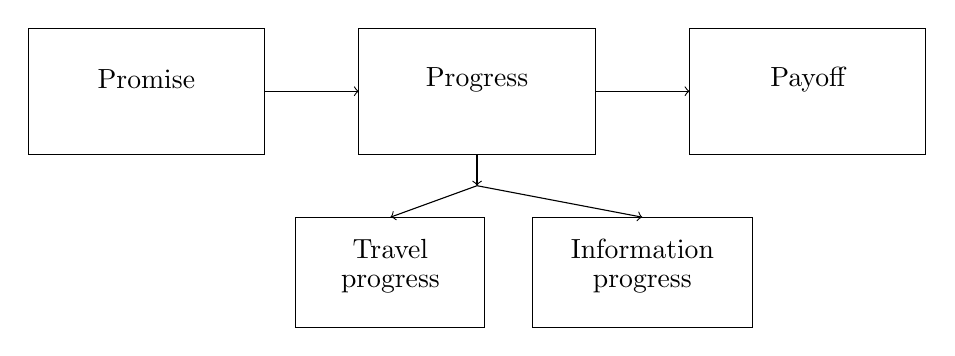
\begin{tikzpicture}
\draw (-5.4,0.8) rectangle (-2.4,-0.8);
\node at (-3.9,0.15) {Promise};

\draw (-1.2,0.8) rectangle (1.8,-0.8);
\node at (0.3,0.15) {Progress};

\draw (3.0,0.8) rectangle (6.0,-0.8);
\node at (4.5,0.15) {Payoff};

\draw[->] (-2.4,0) -- (-1.2,0);
\draw[->] (1.8,0) -- (3.0,0);

\draw (-2.0,-3.0) rectangle (0.4,-1.6);
\node at (-0.8,-2.0) {Travel};
\node at (-0.8,-2.45) {progress};

\draw (1.0,-3.0) rectangle (3.8,-1.6);
\node at (2.4,-2.0) {Information};
\node at (2.4,-2.45) {progress};

\draw[->] (0.3,-0.8) -- (0.3,-1.2);
\draw[->] (0.3,-1.2) -- (-0.8,-1.6);
\draw[->] (0.3,-1.2) -- (2.4,-1.6);
\end{tikzpicture}
\end{figure}

This figure too is a transcript-only schematic. It merely displays the formal separation Sanderson makes between the general narrative triad and the specific channels along which progress can be made legible.

His first example is geographic. In a quest, we move from start to destination, and the reader can watch progress through space:

\begin{equation}
\text{travel progress}:\ \text{start} \to \text{destination}.
\end{equation}

The lecture is careful, however, not to mistake progress for monotone ease. Characters may be diverted, forced backward, or blocked from the path they expected. Still, the direction remains intelligible. The reader knows what it would mean to be closer.

The second example is informational. In a mystery the progress is not primarily spatial; it is a growth in clarity:

\begin{equation}
\text{information progress}:\ \text{few clues} \to \text{more clues} \to \text{clearer picture}.
\end{equation}

False clues, backward steps, and wrong turns are therefore not failures of structure. They belong to the structure, provided they occur inside a channel whose logic is visible.

From here Sanderson arrives at a precise diagnosis of pacing. A story often feels slow not because nothing is happening, but because the promised kind of progress is not being signposted. We cannot feel the motion if we do not know along what axis to measure it.

\begin{equation}
\text{signposted progress} \Rightarrow \text{page-turning momentum}.
\end{equation}

And conversely, if the wrong kind of progress is emphasized, the story can feel stalled even while scenes are active:

\begin{equation}
\text{misaligned signpost} \Rightarrow \text{perceived poor pacing}.
\end{equation}

\subsection{Question \& Answer}

\paragraph{Question.} Why does a story feel slow even when events are happening?

\paragraph{Answer.} Because events alone do not create momentum. Momentum requires a legible channel of progress. If we promise travel, the reader must feel movement through space; if we promise a mystery, the reader must feel accumulating information. When the signposting is weak, or when one channel is promised and another is delivered, the story appears not to move.

This is the strongest formal passage in the lecture. It converts pacing from a vague aesthetic complaint into a failure of stated structure.

\section{Priming the Mind and Writing Ahead of the Page}

The final hack returns from the internal mechanics of story to the daily mechanics of writing. If we are really trying to hit something like \(1{,}700\) words a day, we cannot afford to begin each session by staring into emptiness. Sanderson's solution is to use off-page time to prepare on-page movement.

\begin{equation}
\text{off-page rehearsal} \to \text{on-page execution}.
\end{equation}

The lecture is concrete about the kind of time this means: commutes, workouts, dishes, mowing the lawn, any activity that occupies the body without fully occupying the mind. During that time we do not let attention drift. We ask what the next section of the story should do, what interesting thing could happen, why that scene should matter, why it might become a reader's favorite scene.

\paragraph{A worked routine.} Sanderson's priming method may be written as:
\begin{enumerate}
\item Choose the next scene before the writing session begins.
\item Ask what must happen in it.
\item Ask what would make it vivid rather than routine.
\item Rehearse the scene mentally several times.
\item Sit down already knowing the next stretch of motion.
\end{enumerate}

He even adds a tonal refinement: music may be used to help the imagination settle into the mood of the scene. The point is not decoration but reduction of startup friction. By the time we arrive at the desk, the scene has already begun in the mind.

This advice is then generalized beyond the month-long challenge. Even if our life only leaves real writing time on weekends, commute-time thinking can still prepare the work. The lecture ends, therefore, not by lowering the bar, but by distributing the work more intelligently across the day.

\section{Summary}

Sanderson's five tips form a coherent progression. We begin with a numerical target and a permission structure: write fast, disable the internal editor, but abandon the challenge if it defeats your psychology. We then borrow outer structure, discover inner voice through monologue, generate plot from the gap between wants and needs, organize the whole novel through promise, progress, and payoff, and finally support the daily labor of writing by rehearsing scenes before we reach the page.

The lecture has no board mathematics, yet its procedural mathematics is real. A usable novel can be started by fixing a constraint, extracting a structure, assigning pressure to a character, making progress legible, and reducing the friction between intention and execution. That is the order in which the lecture teaches us to move, and it is also the order in which the notes should allow the reader to think.